\documentclass[12]{article}

../../../../TexScripts/HeaderfileTexDocs.tex

\geometry{left=0.9in, right=0.9in, top=0.9in, bottom=0.9in}

\usepackage{Sweave}
\begin{document}
\Sconcordance{concordance:Project2_Report.tex:Project2_Report.Rnw:%
1 6 1 1 0 17 1 1 166 1 3 29 0 1 2 43 1 1 4 33 0 1 2 2 1 1 53 4 1 1 3 18 %
0 1 3 46 1}

%\SweaveOpts{width='3in',height='3in'}
\doublespacing

\title{Project 2: How different are the academic effects of {\emph{concussion}} versus {\emph{musculoskeletal injury}}?}
\author{Subhrangshu Nandi, UW Madison Department of Statistics \\
Dr. Traci Snedden (PhD, RN, CPNP, CNE), UW Madison School of Nursing
}
%\date{March 13, 2014}
\maketitle
\subsubsection*{Purpose}
To investigate how different the academic effects are, of {\bf{concussion}} and {\bf{musculoskeletal injury}}. 

\subsubsection*{Data}
The data is from a survey send out to a large groups of undergraduate students at a large midwestern 
university. Overall response rate of the survey was $6.72\%$ (1,950 out of 29,000). The response rate is slightly lower than the average response rate for external surveys which is around 10-15\%. Out of 1,950 respondents, 76 of them reported to have had a concussion and 168 of them reported to have had a musculoskeletal injury during since starting college. 


% latex table generated in R 3.3.1 by xtable 1.8-2 package
% Mon Mar 27 10:53:03 2017
\begin{table}[htbp]
\centering
\begin{tabular}{lrr}
  \hline
 & Concussion & Musculoskeletal \\ 
  \hline
N & 76 & 168 \\ 
  N (males) & 21 & 50 \\ 
  N (females) & 55 & 117 \\ 
  Average Age & 20.18 & 20.57 \\ 
  Std Dev Age & 2.37 & 2.95 \\ 
  American Indian or Alaska Native & 0 & 0 \\ 
  Asian & 6 & 12 \\ 
  Black or African American & 1 & 1 \\ 
  Others & 4 & 3 \\ 
  White & 61 & 152 \\ 
  Hispanic or Latino or Spanish Origin & 3 & 4 \\ 
  Not Hispanic or Latino or Spanish Origin & 70 & 154 \\ 
  TotalDays & 328 & 500 \\ 
  ADHD/ADD & 3 & 1 \\ 
  Learning Disability & 1 & 2 \\ 
  Psychiatric Disorder & 11 & 26 \\ 
  Migraine Headaches & 9 & 12 \\ 
  None & 43 & 114 \\ 
   \hline
\end{tabular}
\caption{Demographics of Injury Types} 
\label{tab:Tab0Table1}
\end{table}
\subsection*{Methods}
The students were asked several questions to assess how their injuries affected their academics. They were asked to respond how strongly they agreed or disagreed with the questions. The responses were recorded in 1 through 5 (Likert scale), where 1 being ``strongly disagree'' and 5 being ``strongly agree''. The questions were designed to assess the adverse consequences of their injuries. A higher numeric ( 4 or 5 ) response indicated more severe effect of the injury. For each question, two statistical tests were conducted to asses the difference in academic effects, of concussion and musculoskeletal injury. \\
\noindent
{\bf{$\chi^2$ test of independence}}: To test of the responses were independent of the injury type. The null hypothesis is that the proportions of five numeric responses (of agreement) were the same in the two types of injuries. If the p-value < 0.05 for an academic aspect, we rejected this null hypothesis and concluded that the injuries did have different impact on that particular academic aspect. 
\begin{eqnarray}
\nonumber
\text{H}_0&:& \text{Responses were independent of injury type} \\
\text{H}_a&:& \text{Responses were not independent of injury type} 
\label{eq:chiSqTest}
\end{eqnarray}
\noindent
{\emph{Assumptions}}:
\begin{itemize}
\item Simple random sample: The sample data is a random sampling from a fixed distribution or  population where every collection of members of the population of the given sample size has an equal probability of selection. Here this assumption is violated, so caution should be exercised when extrapolating the findings to all students.
\item Sample size: A sample with a sufficiently large size is assumed. If a $\chi^2$ test is conducted on a sample with a smaller size, then the $\chi^2$ test will yield an inaccurate inference by increasing Type II error.
\item Expected cell count: Adequate expected cell counts. Some require 5 or more, and others require 10 or more. A common rule is 5 or more in all cells of a 2-by-2 table, and 5 or more in 80\% of cells in larger tables, but no cells with zero expected count. When this assumption is not met, Yates's correction is applied.
\item Independence: The observations are always assumed to be independent of each other. This means $\chi^2$ cannot be used to test correlated data (like matched pairs or panel data).
\end{itemize}
\noindent
{\bf{One-sided $T$ test of mean scores}}: To test if the mean responses of students with ``concussion'' were higher than those of ``musculoskeletal'' injuries. If the p-value < 0.05 for an academic aspect, we rejected this null hypothesis and concluded that the effect of concussion on that academic aspect was higher than musculoskeletal injury.
\begin{eqnarray}
\nonumber
\text{H}_0&:& \mu_{\text{concussion}} = \mu_{\text{musculoskeletal}} \\
\text{H}_a&:& \mu_{\text{concussion}} \ne \mu_{\text{musculoskeletal}}
\label{eq:tTest}
\end{eqnarray}
{\emph{Assumptions}}:
\begin{itemize}
\item Normality: Each of the two populations being compared should follow a normal distribution. 
\item Independence: The data used to carry out the test should be sampled independently from the two populations being compared. 
\end{itemize}

\noindent
{\bf{Regression Model for Academic Effects}}: The responses to the questions on academic effects were all added up to form one ``Academic Effect'' variable, (i.e., a composite Likert scale). Higher values of this variable indicated more severe academic impact. To estimate the difference in academic effects, of the two types of injuries, concussion and musculoskeletal, a regression model was fit, as in eq \ref{eq:Reg}. The response variable ($y$) was the composite academic effect. The covariates ($x_1, \dots, x_p$) were injury type, along with demographic factors such as age, gender, race, ethnicity, academic status (years in college), history of mental illness, such as ADHD, learning disability, etc, and interactions of the factors.

\begin{equation} 
y = \beta_0 + \beta_1x_1 + \dots + \beta_p x_p + \epsilon 
\label{eq:Reg}
\end{equation}

\subsection*{Results}
Table \ref{tab:Tab1Summary} is a summary of the two tests conducted on each question regarding academic effect

% latex table generated in R 3.3.1 by xtable 1.8-2 package
% Mon Mar 27 10:53:03 2017
\begin{table}[htbp]
\centering
\begin{tabular}{llrrr}
  \hline
 & Question & Chi-sq p & t-test p & mean diff \\ 
  \hline
Q5.3\_1 & I forget what has been said in class & 0.0002 & 0.000 & -0.64 \\ 
  Q5.3\_2 & I get overwhelmed when studying & 0.0013 & 0.000 & -0.76 \\ 
  Q5.3\_3 & I get overwhelmed in class & 0.0009 & 0.001 & -0.54 \\ 
  Q5.3\_4 & I get nervous before tests & 0.0007 & 0.000 & -0.72 \\ 
  Q5.3\_5 & I have trouble managing my time & 0.0006 & 0.000 & -0.64 \\ 
  Q5.3\_6 & I have difficulty taking notes while in a lecture class & 0.0043 & 0.000 & -0.6 \\ 
  Q5.3\_7 & I am late to class & 0.3989 & 0.576 & 0.03 \\ 
  Q5.3\_8 & I have trouble prioritizing assignments and meeting deadlines & 0.0011 & 0.000 & -0.61 \\ 
  Q5.3\_9 & Others do not understand my problems & 0.0024 & 0.090 & -0.25 \\ 
  Q5.3\_10 & I procastinate on things I need to do & 0.0003 & 0.000 & -0.99 \\ 
  Q5.3\_11 & I have to review materials more than I used to & 0.0021 & 0.001 & -0.54 \\ 
  Q5.3\_12 & I dont always understand instructions for assignments & 0.0244 & 0.002 & -0.49 \\ 
  Q5.3\_13 & I need extra time to complete assignments & 0.0358 & 0.007 & -0.39 \\ 
  Q5.3\_14 & I have difficulty putting my thoughts into words & 0.0000 & 0.000 & -0.75 \\ 
  Q5.3\_15 & I have trouble reading books or magazines & 0.0001 & 0.001 & -0.47 \\ 
  Q5.3\_16 & I have trouble paying attention in class & 0.0000 & 0.000 & -0.91 \\ 
  Q5.3\_17 & I have trouble paying attention while studying & 0.0000 & 0.000 & -1.04 \\ 
  Q5.3\_18 & I have trouble doing work on a computer or other mobile device & 0.0006 & 0.000 & -0.66 \\ 
  Q5.3\_19 & I cant study for as long as I used to prior to my injury & 0.0026 & 0.000 & -0.53 \\ 
  Q5.3\_20 & I get headaches when I read or write & 0.0004 & 0.000 & -0.65 \\ 
  Q5.3\_21 & I need extra time to complete assignments & 0.0014 & 0.002 & -0.44 \\ 
  Q5.3\_22 & I have fewer friends than before my injury & 0.0820 & 0.030 & -0.24 \\ 
   \hline
\end{tabular}
\caption{Statistical tests of responses} 
\label{tab:Tab1Summary}
\end{table}
The results of the $\chi^2$ test shows that all questions, except Q5.3\_7 and Q5.3\_22 have statistically significant difference in responses, when compared between students with concussion and musculoskeletal injury. The t-test p-values confirm that in all aspects (except Q5.3\_7), the academic effect of concussion is much more severe than that of musculoskeletal injury. Q5.3\_17 has the largest effect size (-1.04). The effect of concussion on that academic aspect is the maximum. 


\noindent
{\bf{ Regression Model Fit}}\\
In the final dataset for the model, there were 60 students who reported concussion and 125 students who reported musculoskeletal injury. The lower numbers were due to removing of non-reponses in all the covariates included in the model. For example, there were 58 students who did not answer any of the questions related to academic effects. There was 1 student who did not respond to the question on gender. After performing backward elimination, the final model had gender, academic status as the controlling demographic factors along with the predictor variable injury type. 

% latex table generated in R 3.3.1 by xtable 1.8-2 package
% Mon Mar 27 10:53:03 2017
\begin{table}[H]
\centering
\begin{tabular}{lrrrr}
  \hline
 & B & SE\_B & beta & pValue \\ 
  \hline
Intercept & 51.45 & 3.77 & 0.00 & 0.0000 \\ 
  Gender: Female & -4.84 & 2.89 & -0.12 & 0.0956 \\ 
  Academic Status: completed 1-2 yrs & 8.83 & 4.38 & 0.16 & 0.0453 \\ 
  Academic Status: completed 2-3 yrs & 1.41 & 3.79 & 0.03 & 0.7101 \\ 
  Academic Status: completed 3-4 yrs & -3.95 & 3.71 & -0.09 & 0.2887 \\ 
  Academic Status: completed 4 or more yrs & 7.25 & 4.91 & 0.12 & 0.1417 \\ 
  Injury Type: Musculoskeletal & -12.70 & 2.85 & -0.31 & 0.0000 \\ 
   \hline
\end{tabular}
\caption{Regression results of academic effects of inury type} 
\label{tab:Tab2Reg}
\end{table}
Multiple regression analysis was used to test if the injury type significantly predicted participants' academic effects. The results of the regression indicated that injury type, along with two demographic  covariates explained 16.09\% of the variance ($R^2=0.16, F(6,178) = 5.687, p < 0.01$). Table \ref{tab:Tab2Reg} shows the regression results, with both unstandardized and standardized betas, along with standard errors of beta and the p-values. Injury type is statistically significant ($\beta = 12.70, p < 0.01$). Students with concussion had, on an average 12.70 higher (hence more severe) academic effect compared to students with musculoskeletal injury. Gender was also a significant predictor. Male students, on an average had worse academic effect, ($\beta = 4.84, p < 0.1$). Students who completed 1-2 years of college had worse academic effect ($\beta = 8.83, p < 0.05$) compared to students in their first year of college. Tukey's post-hoc test was conducted on the academic status variable to detect any difference between any other subgroups. The post-hoc test revealed that students who completed 1-2 yrs had worse academic effects than students who completed 3-4 yrs ($\beta = 14.13, p < 0.05$). There was no statistically significant difference between any other groups.  


% Below are bar plots of the responses to the questions.
% \begin{figure}[H]
% 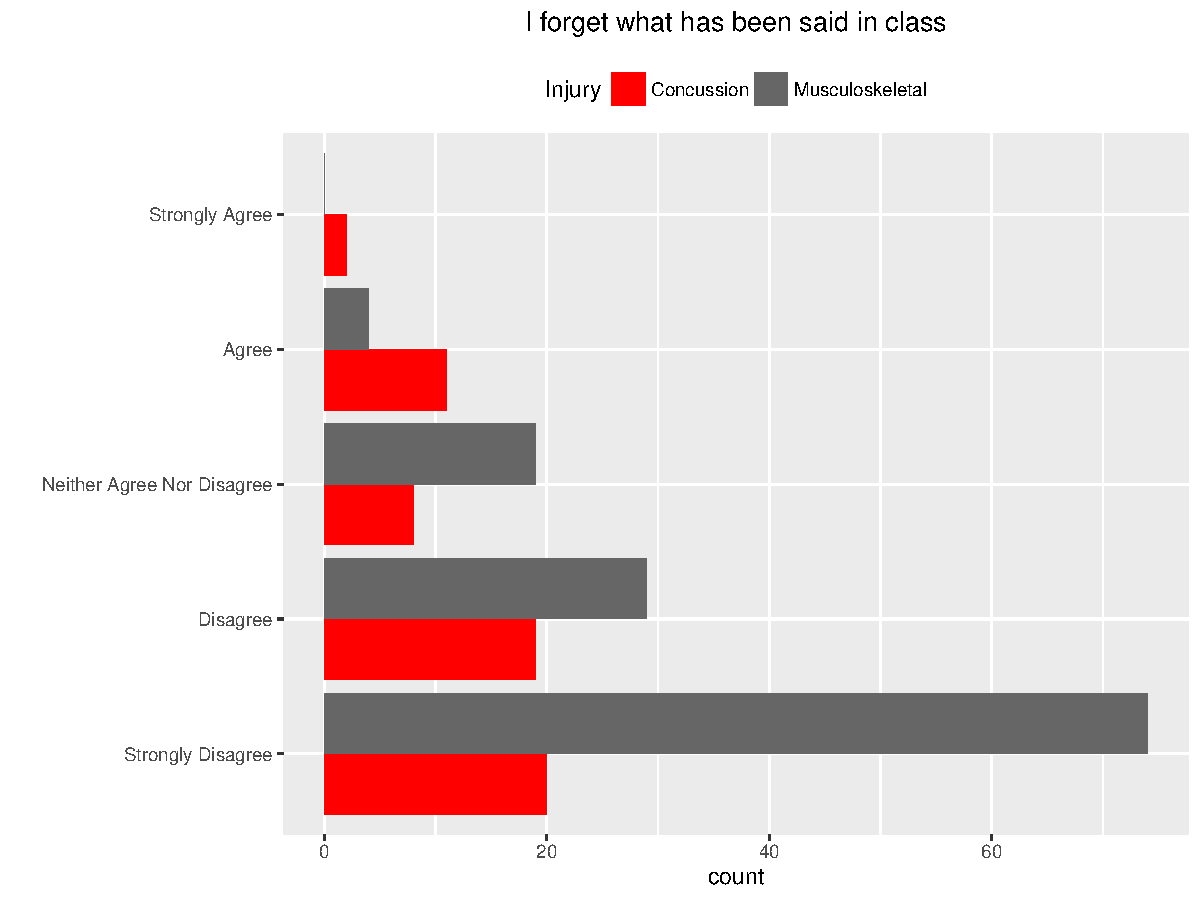
\includegraphics[width=0.5\linewidth]{Q5_3_1_barPlot.pdf}
% 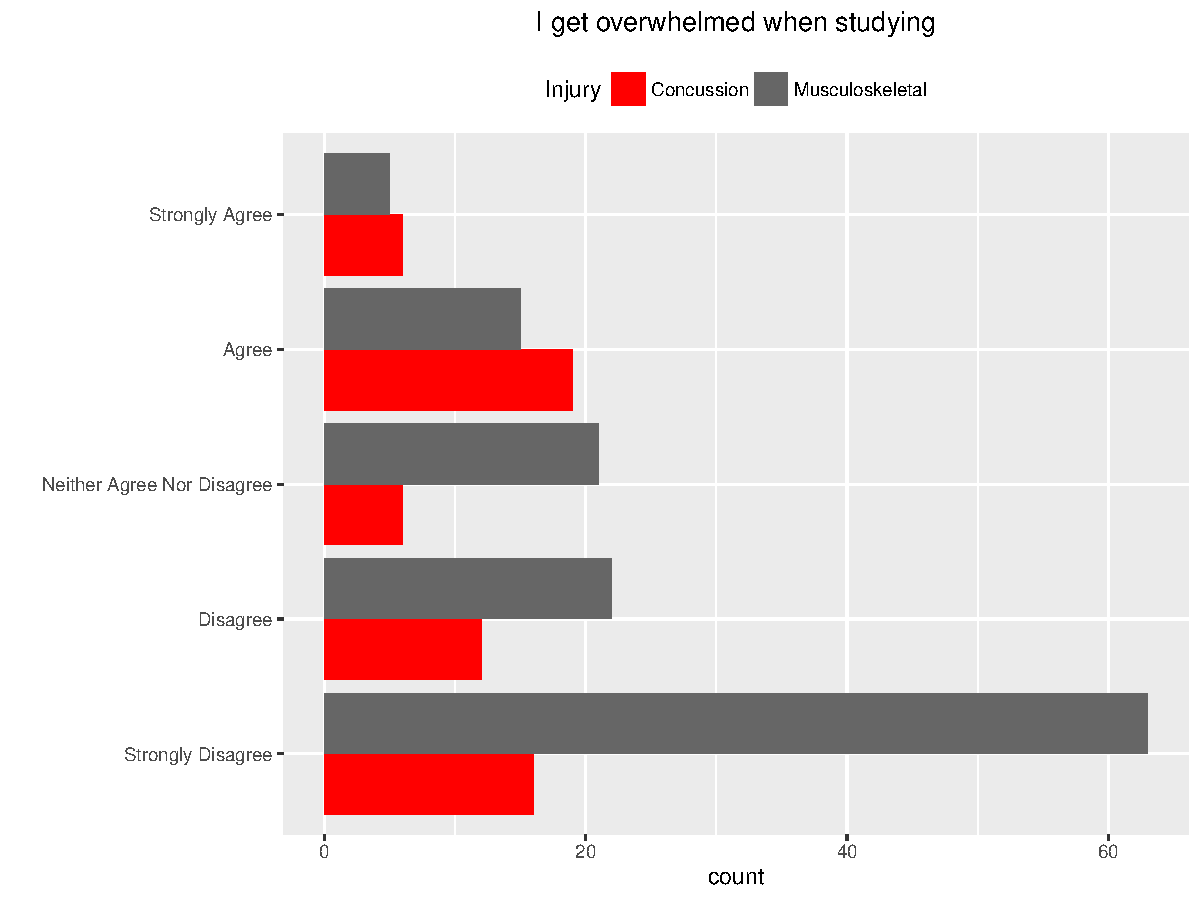
\includegraphics[width=0.5\linewidth]{Q5_3_2_barPlot.pdf} \\
% 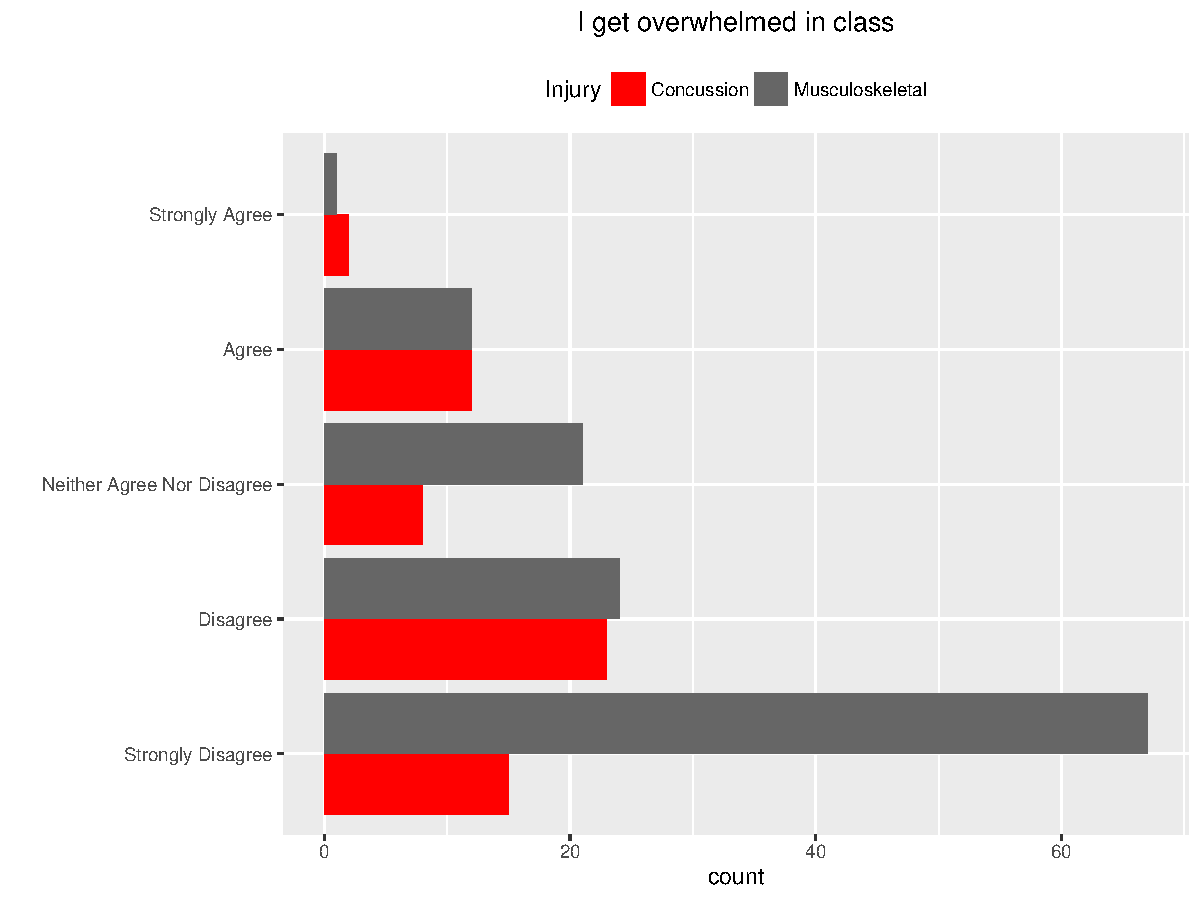
\includegraphics[width=0.5\linewidth]{Q5_3_3_barPlot.pdf} 
% 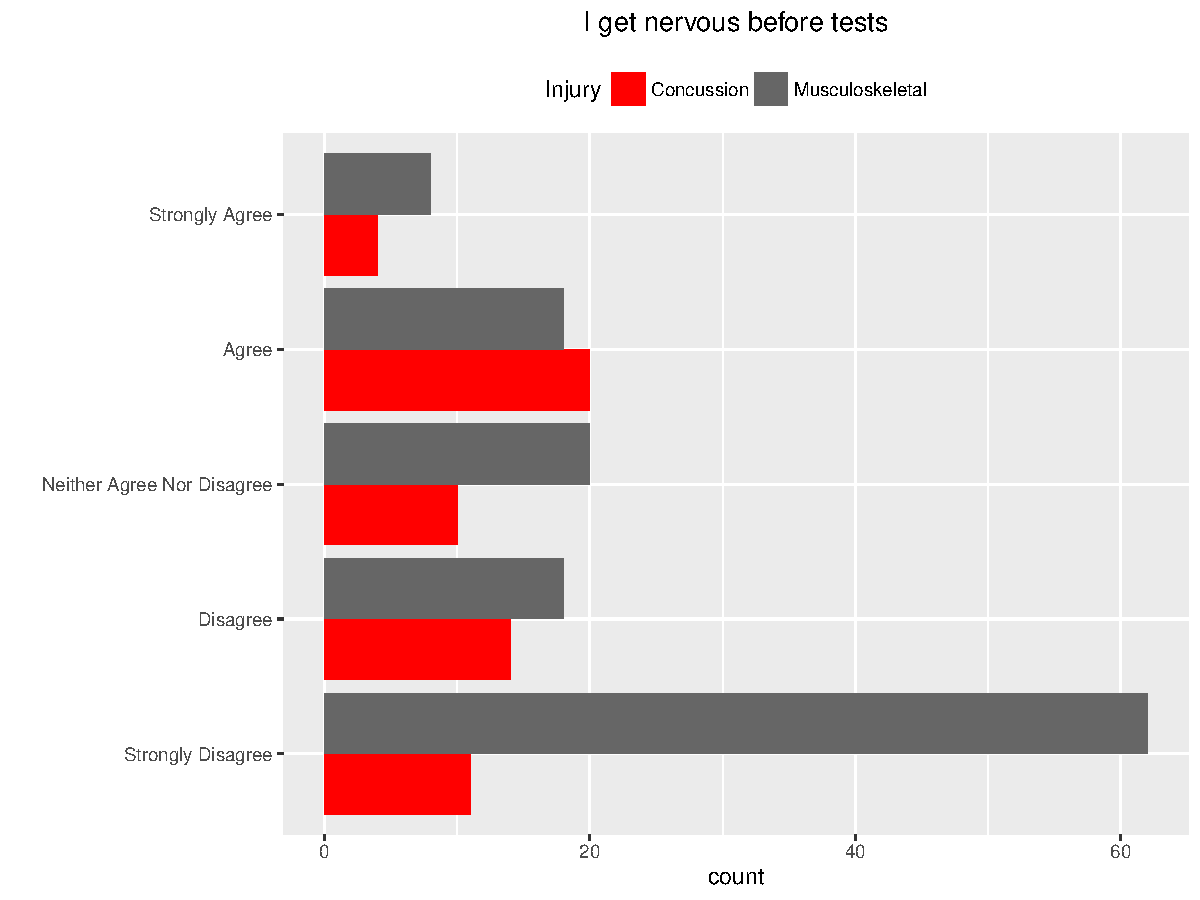
\includegraphics[width=0.5\linewidth]{Q5_3_4_barPlot.pdf} \\
% 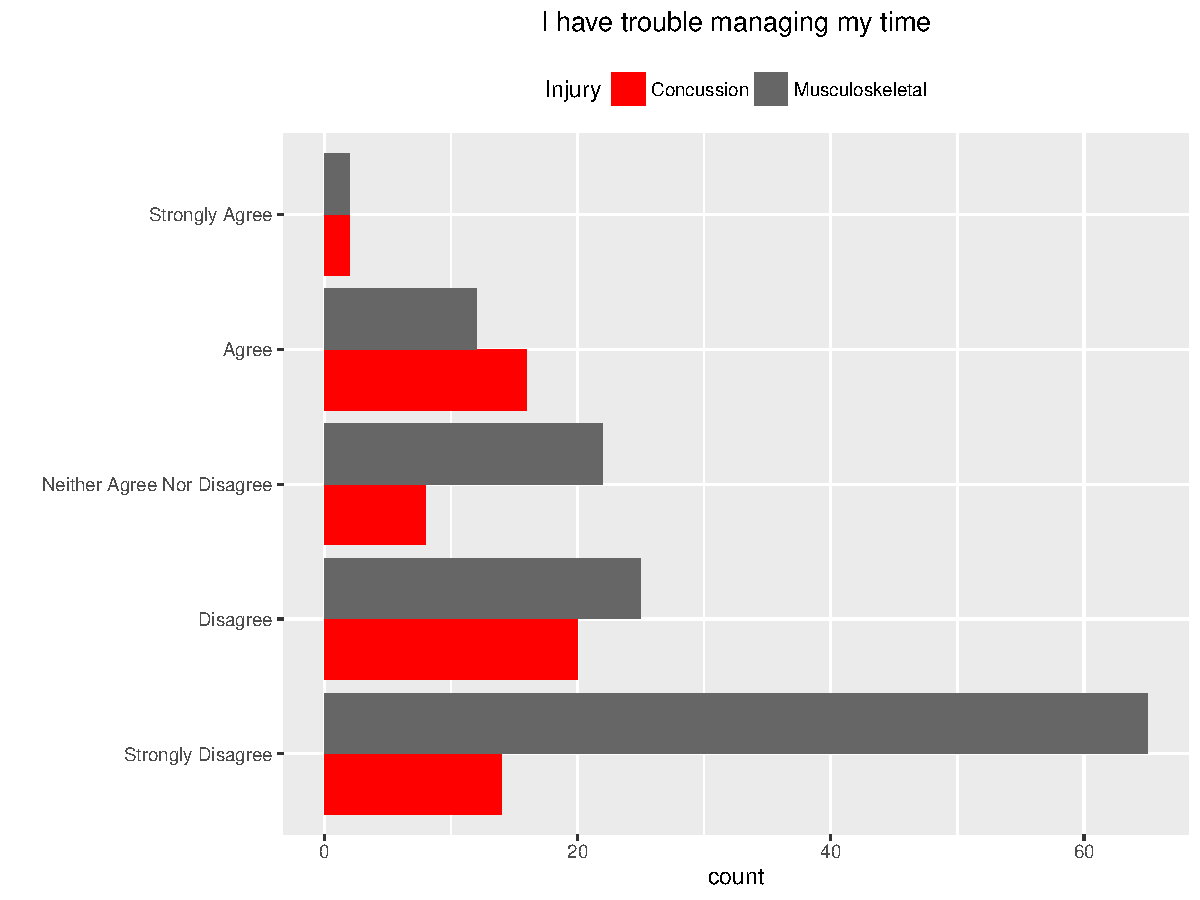
\includegraphics[width=0.5\linewidth]{Q5_3_5_barPlot.pdf}
% 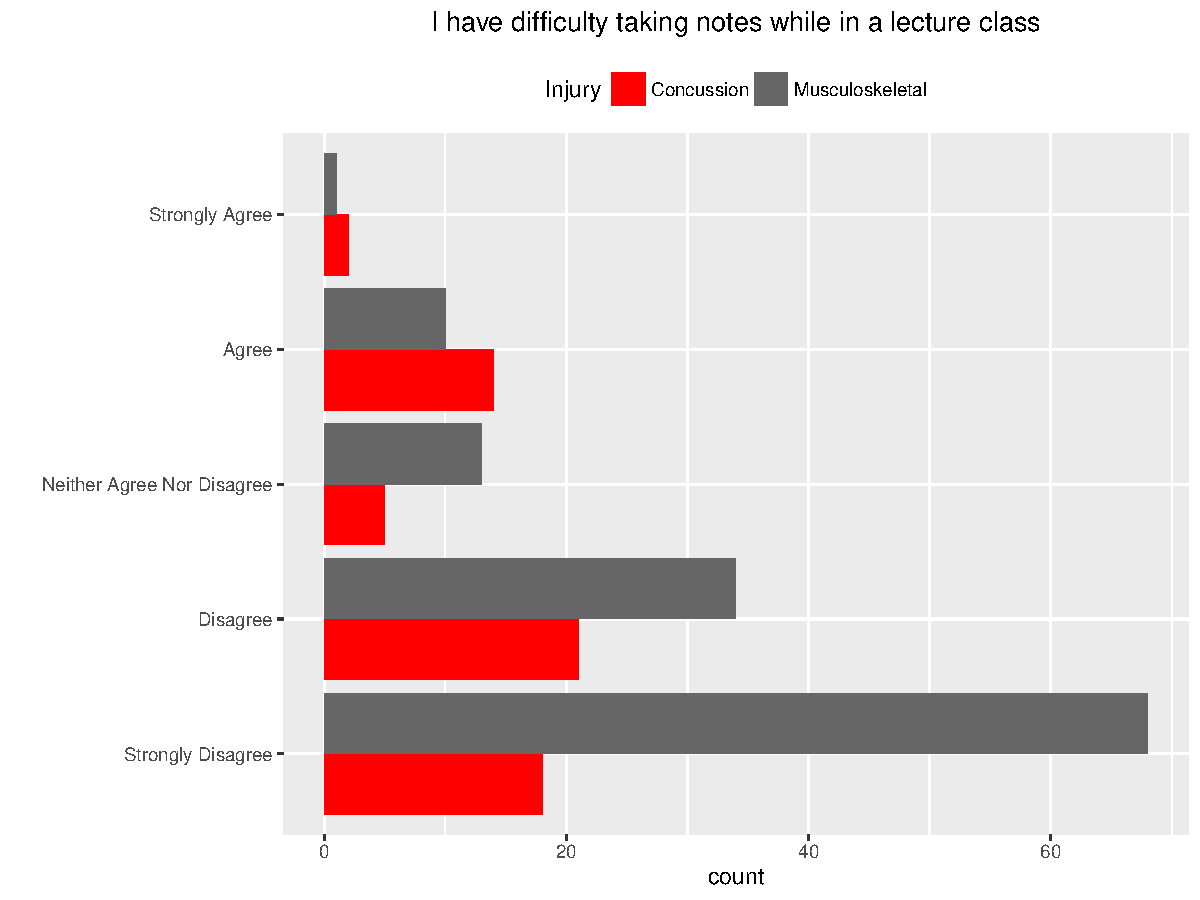
\includegraphics[width=0.5\linewidth]{Q5_3_6_barPlot.pdf}
% \end{figure}
% 
% \begin{figure}[H]
% 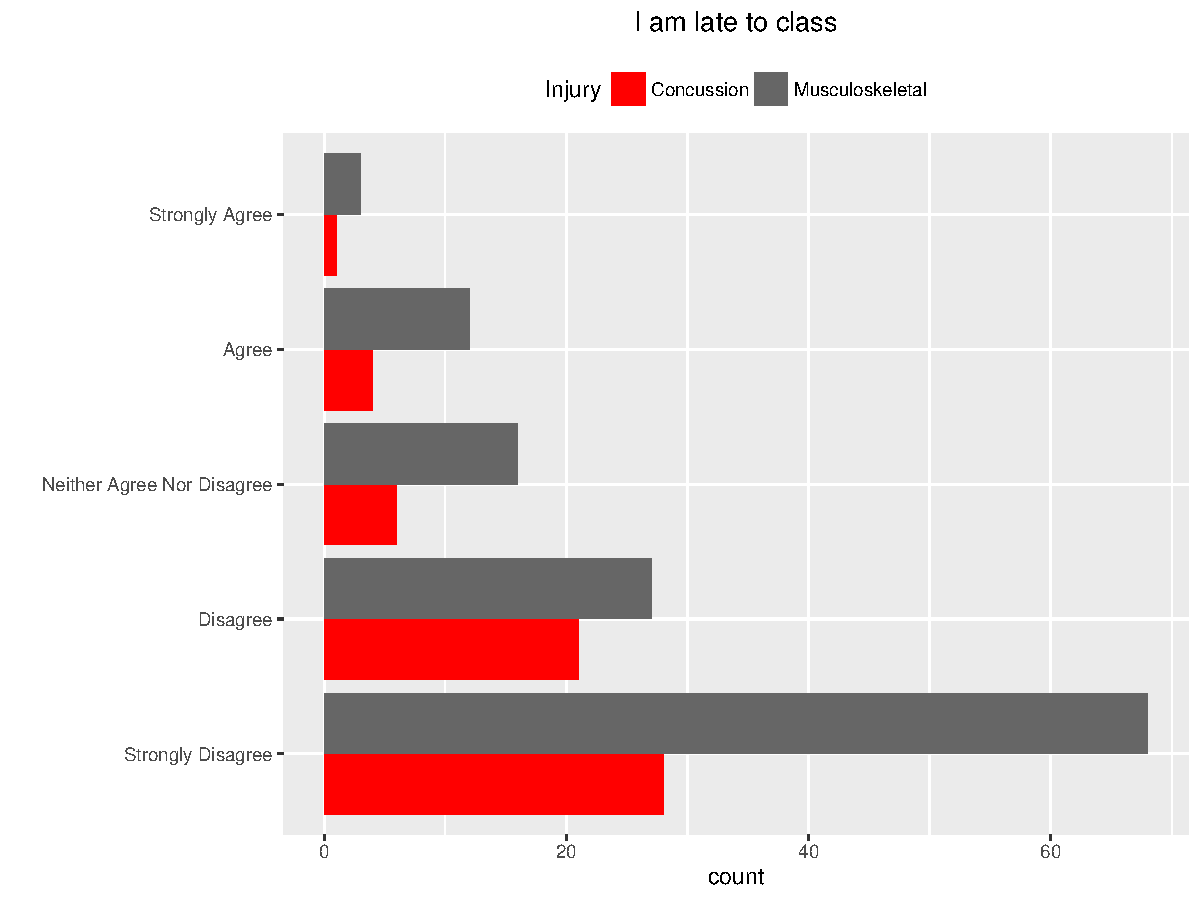
\includegraphics[width=0.5\linewidth]{Q5_3_7_barPlot.pdf} 
% 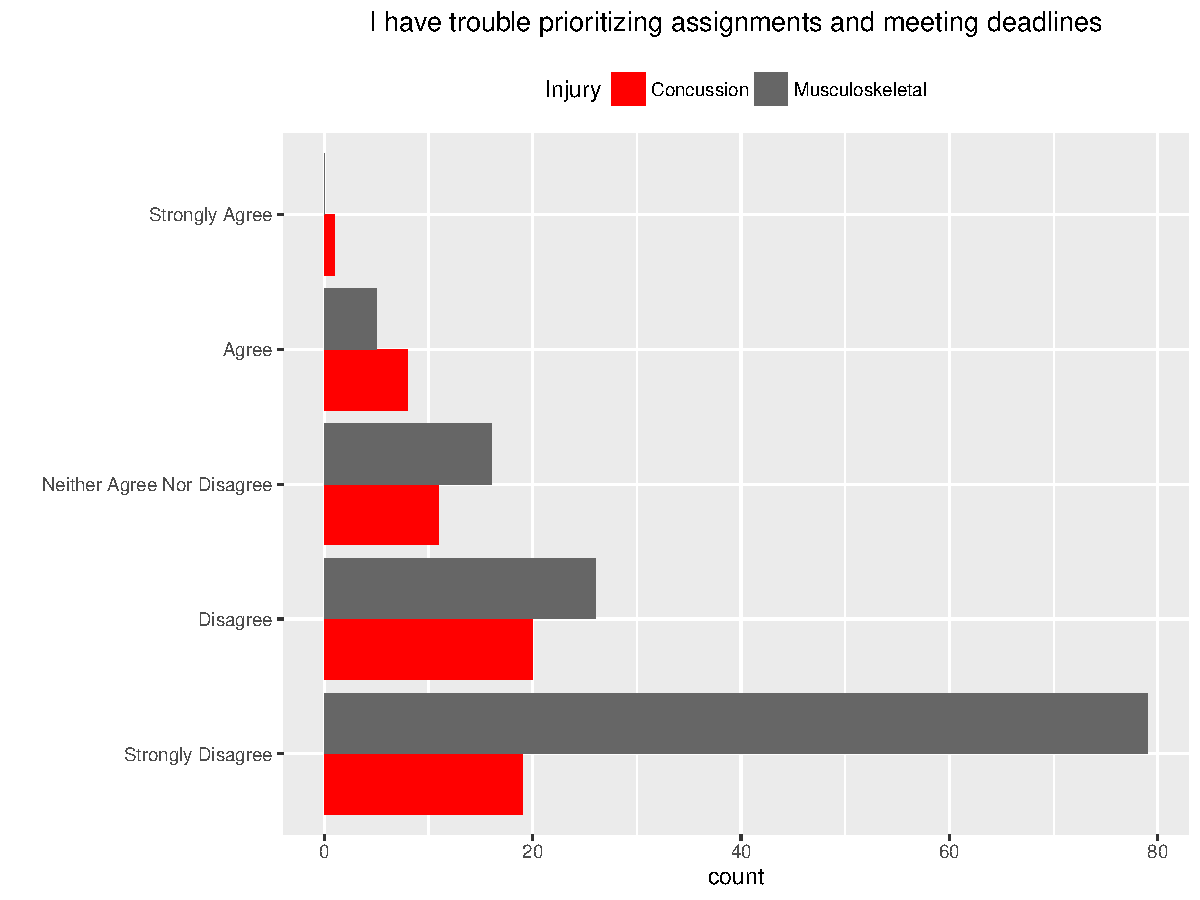
\includegraphics[width=0.5\linewidth]{Q5_3_8_barPlot.pdf} \\
% 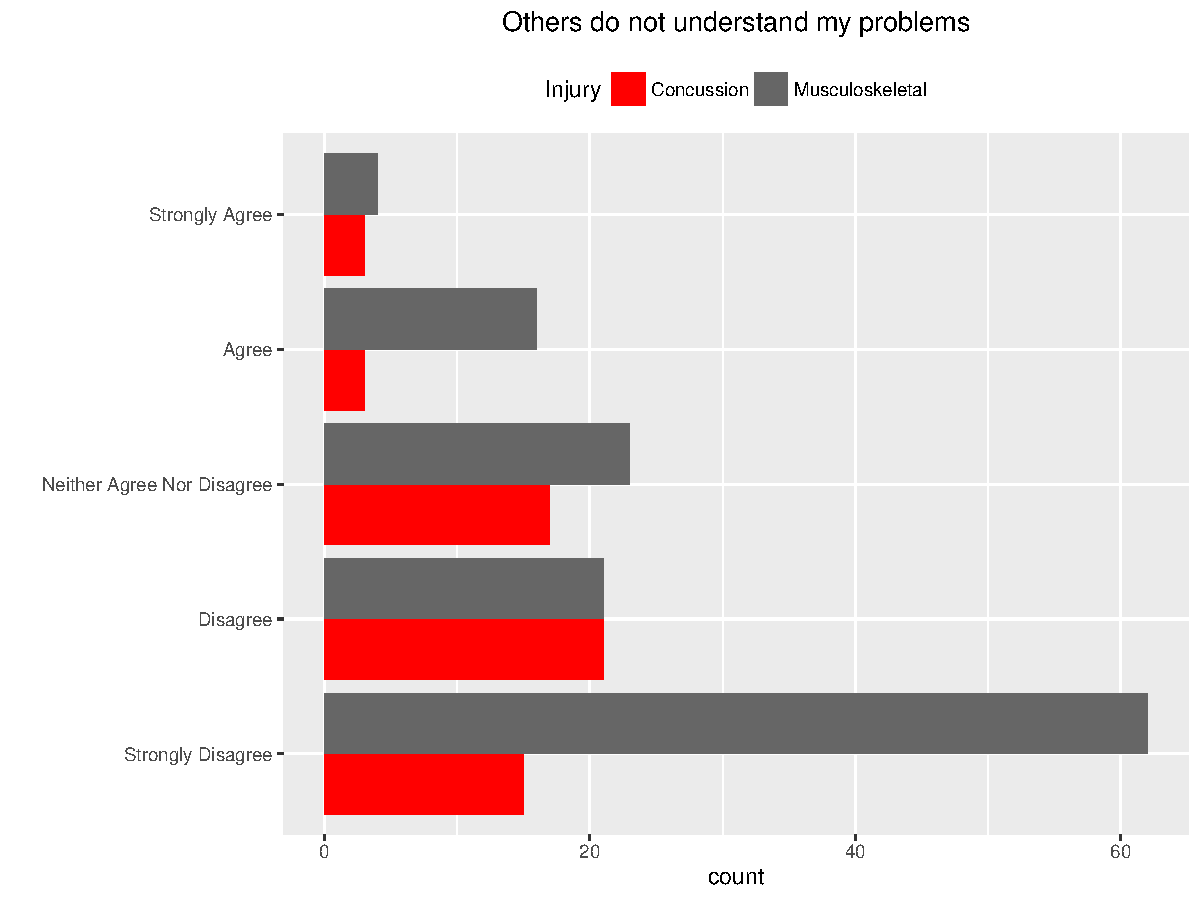
\includegraphics[width=0.5\linewidth]{Q5_3_9_barPlot.pdf}
% 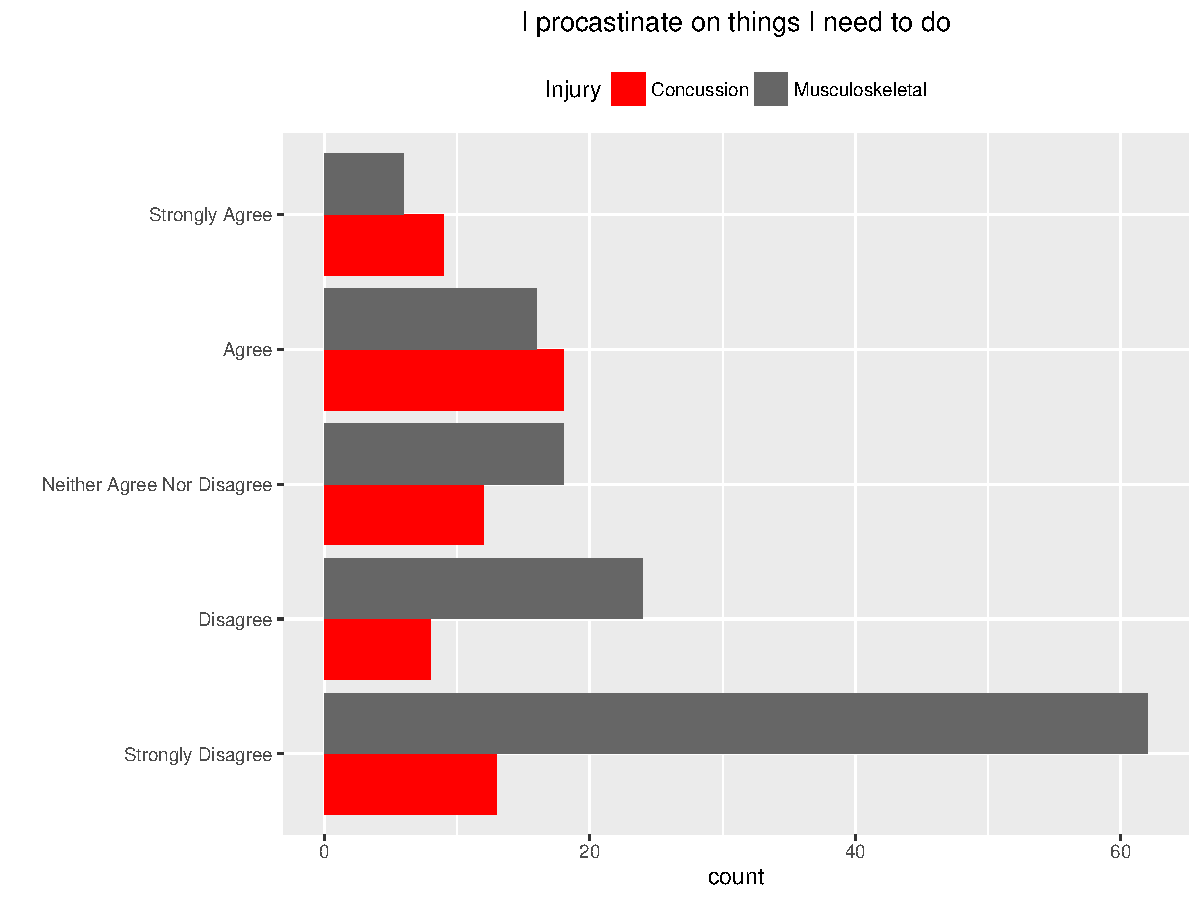
\includegraphics[width=0.5\linewidth]{Q5_3_10_barPlot.pdf} \\
% 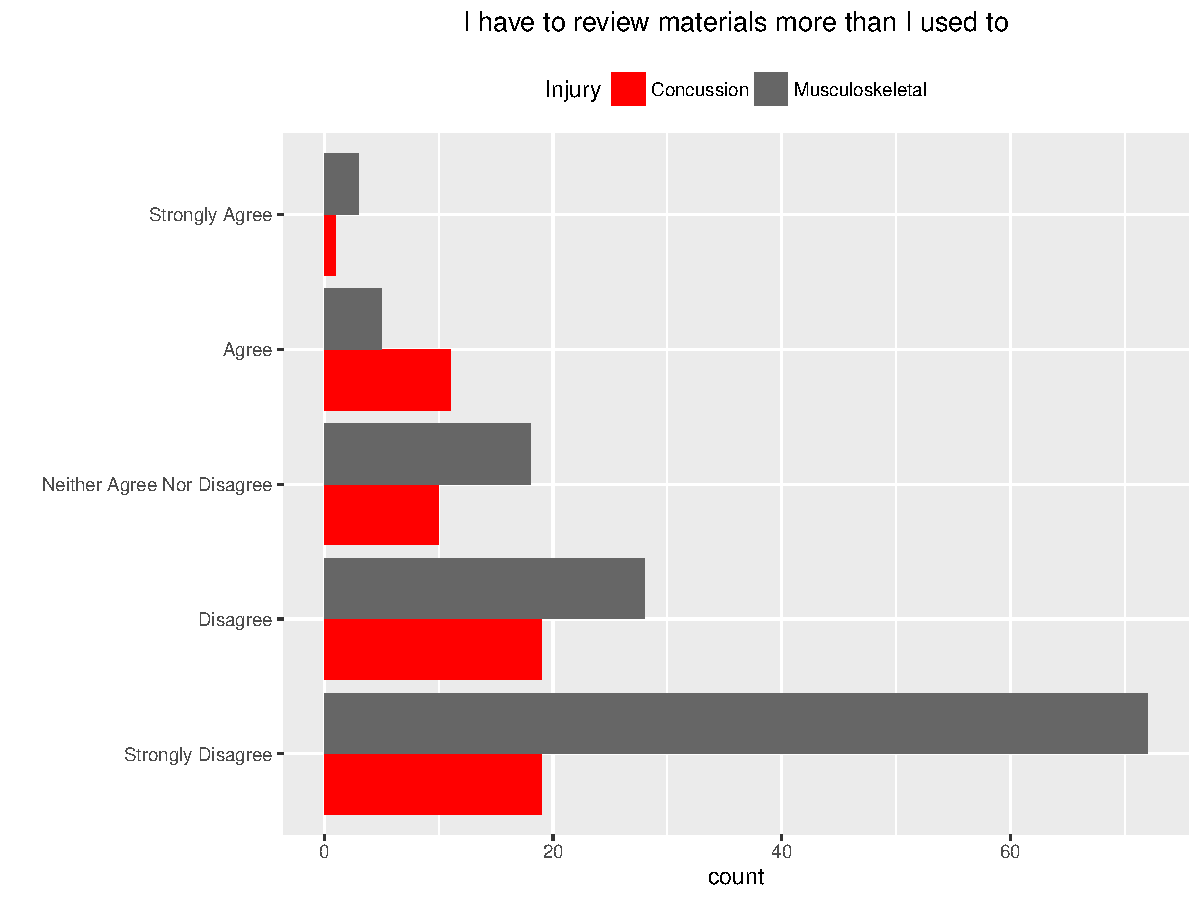
\includegraphics[width=0.5\linewidth]{Q5_3_11_barPlot.pdf}
% 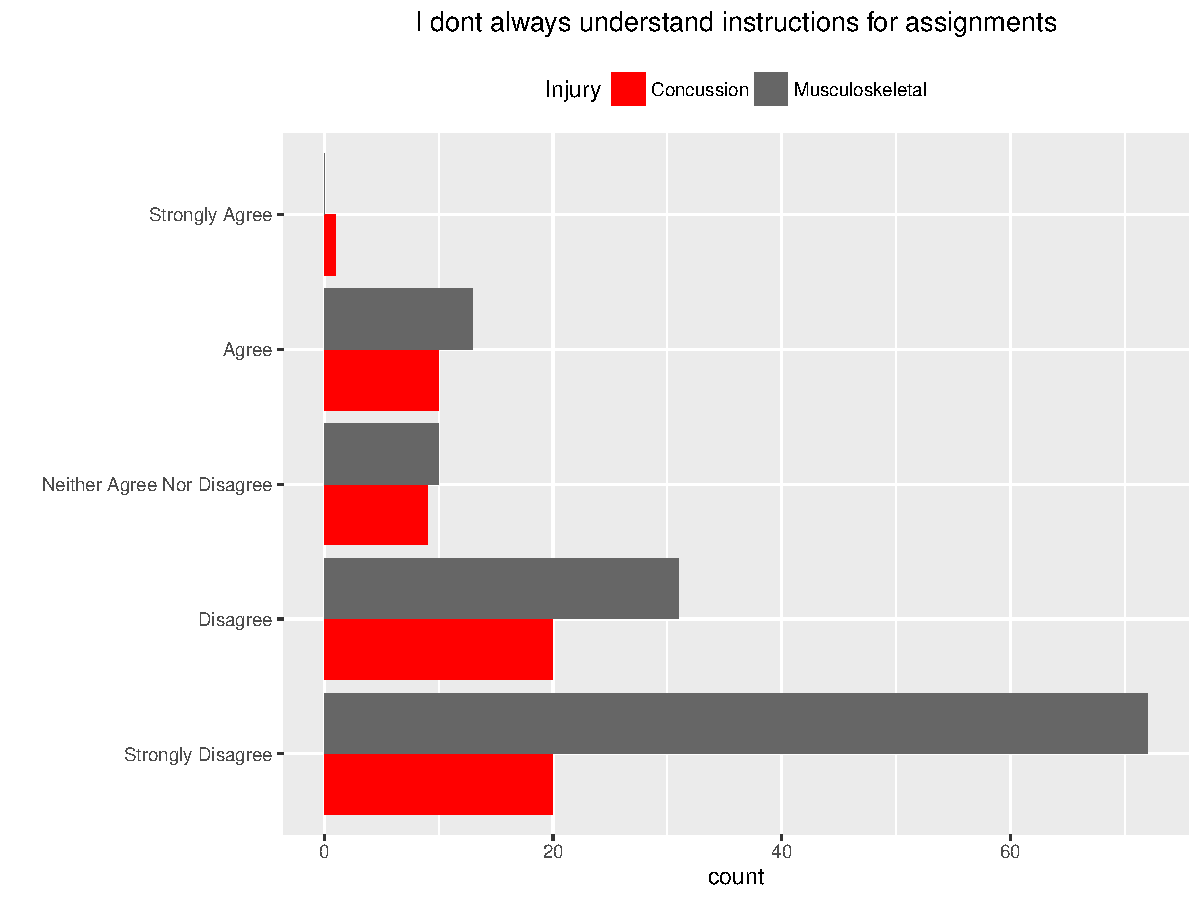
\includegraphics[width=0.5\linewidth]{Q5_3_12_barPlot.pdf} \\
% \end{figure}
% 
% \begin{figure}[H]
% 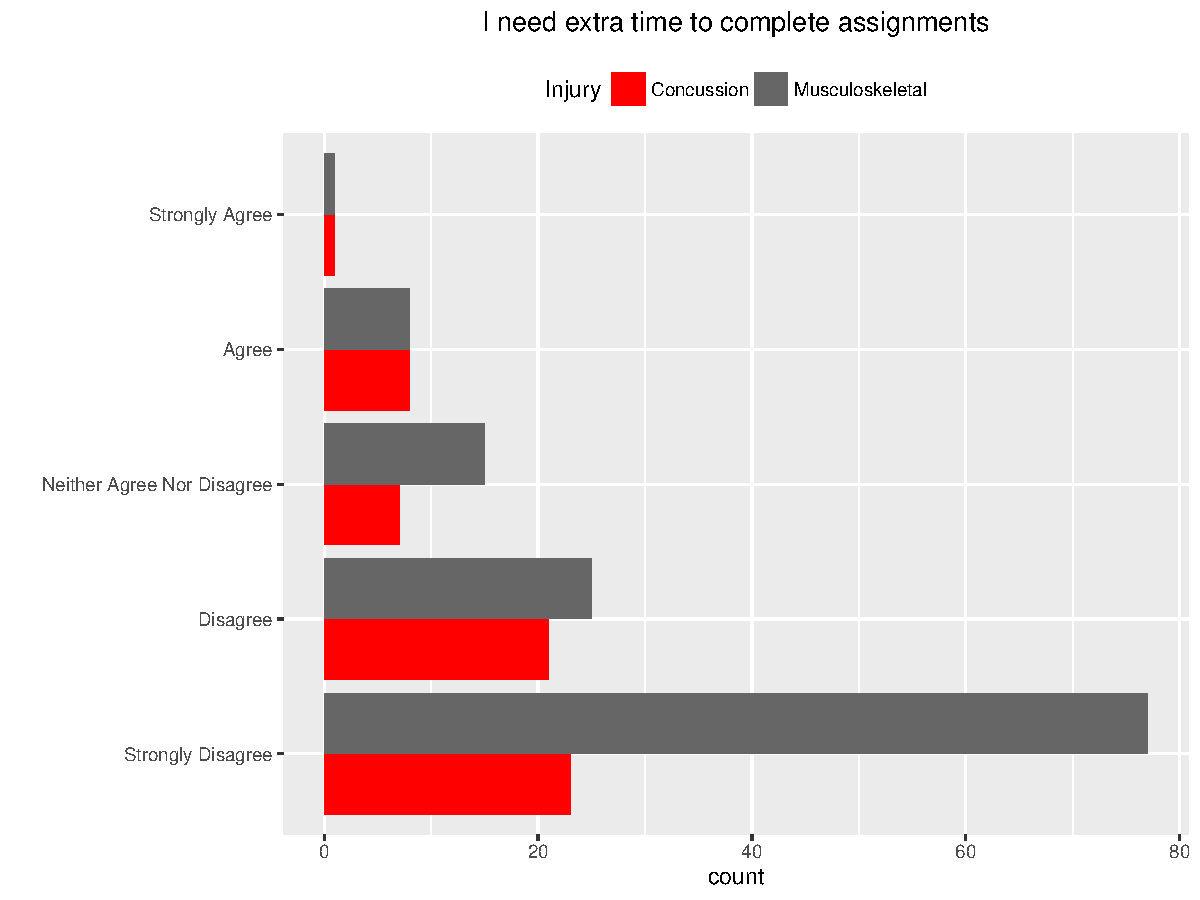
\includegraphics[width=0.5\linewidth]{Q5_3_13_barPlot.pdf}
% 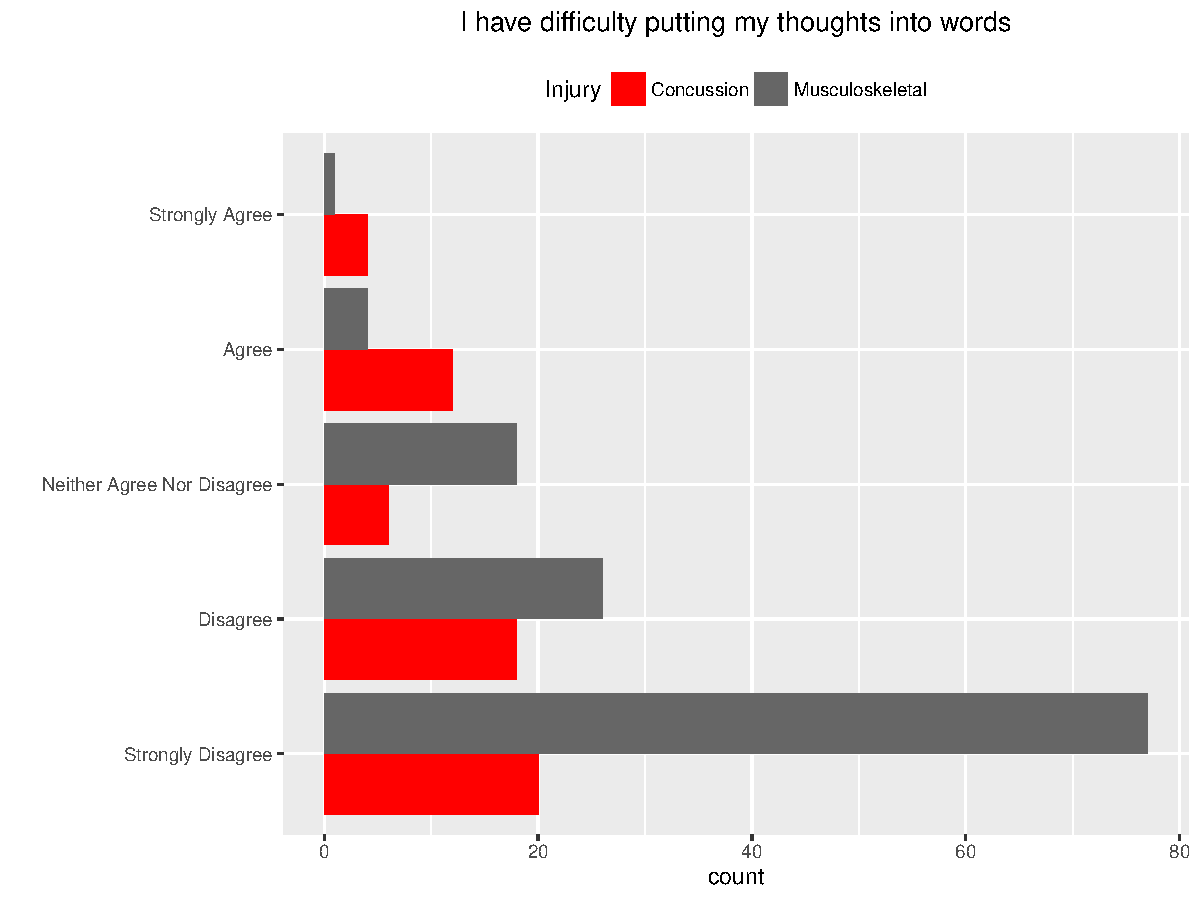
\includegraphics[width=0.5\linewidth]{Q5_3_14_barPlot.pdf} \\
% 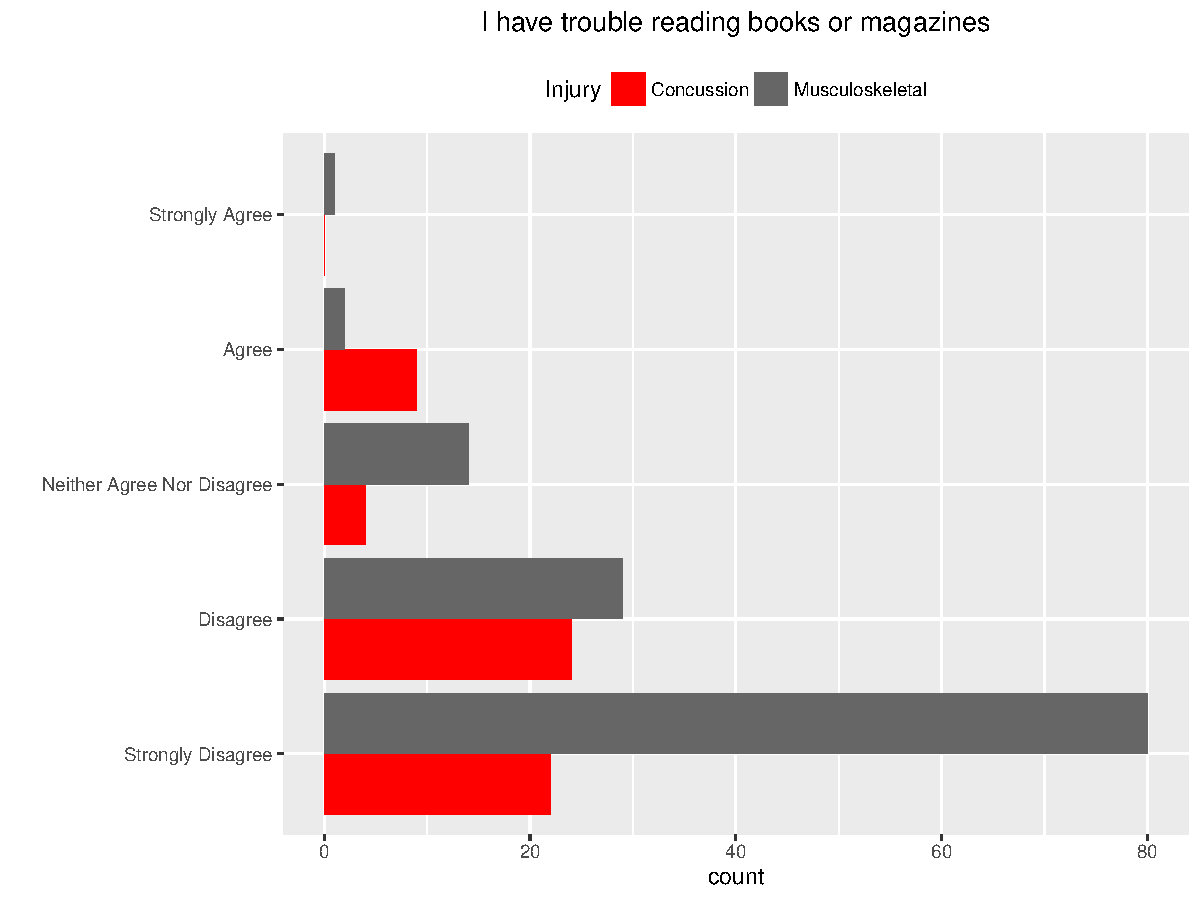
\includegraphics[width=0.5\linewidth]{Q5_3_15_barPlot.pdf}
% 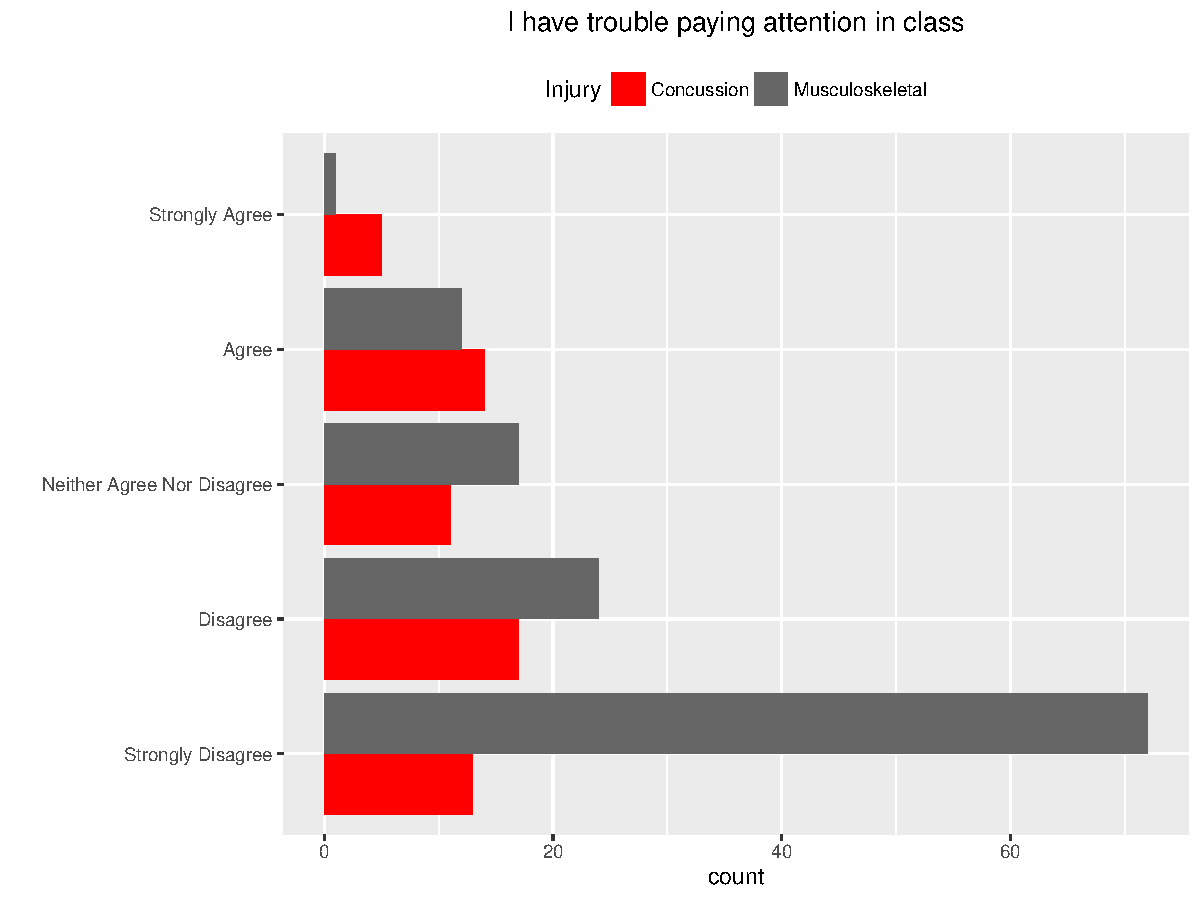
\includegraphics[width=0.5\linewidth]{Q5_3_16_barPlot.pdf} \\
% 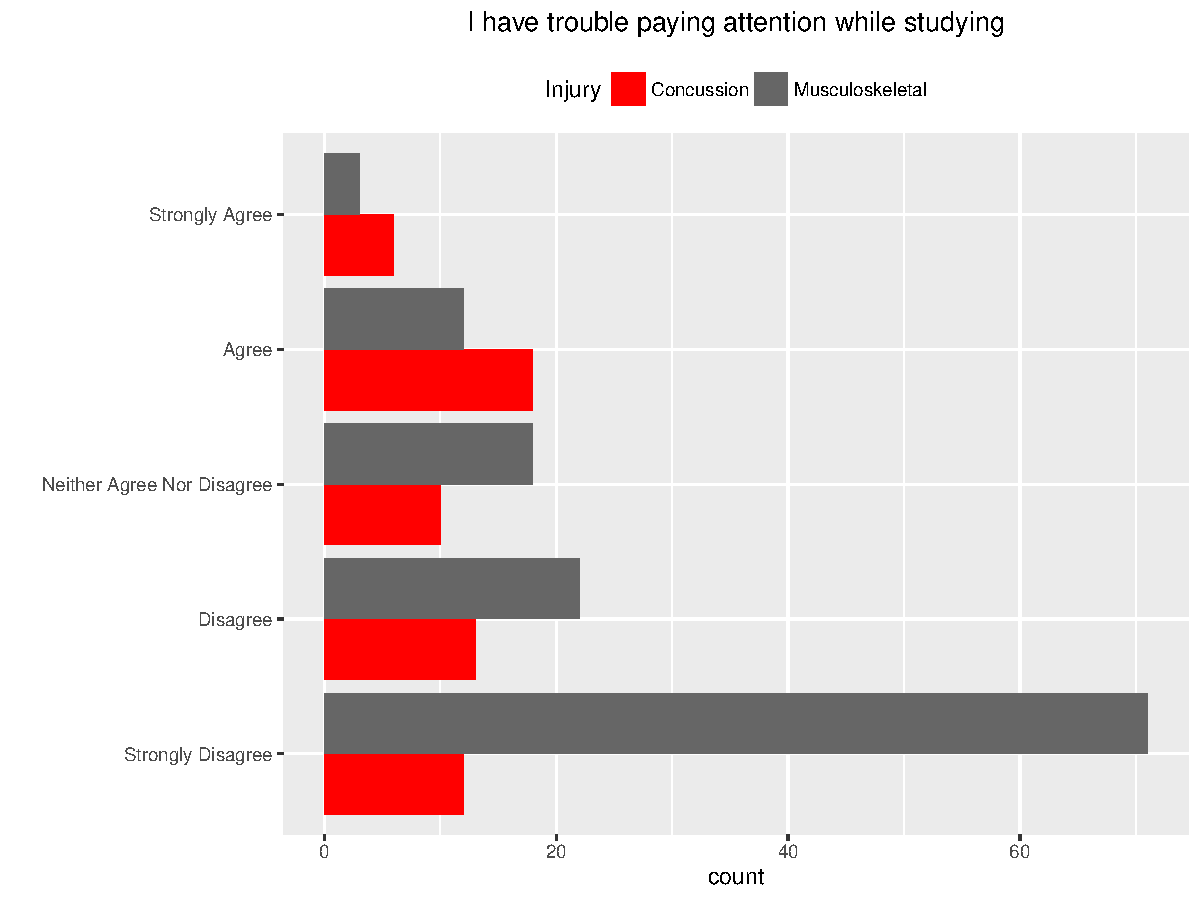
\includegraphics[width=0.5\linewidth]{Q5_3_17_barPlot.pdf}
% 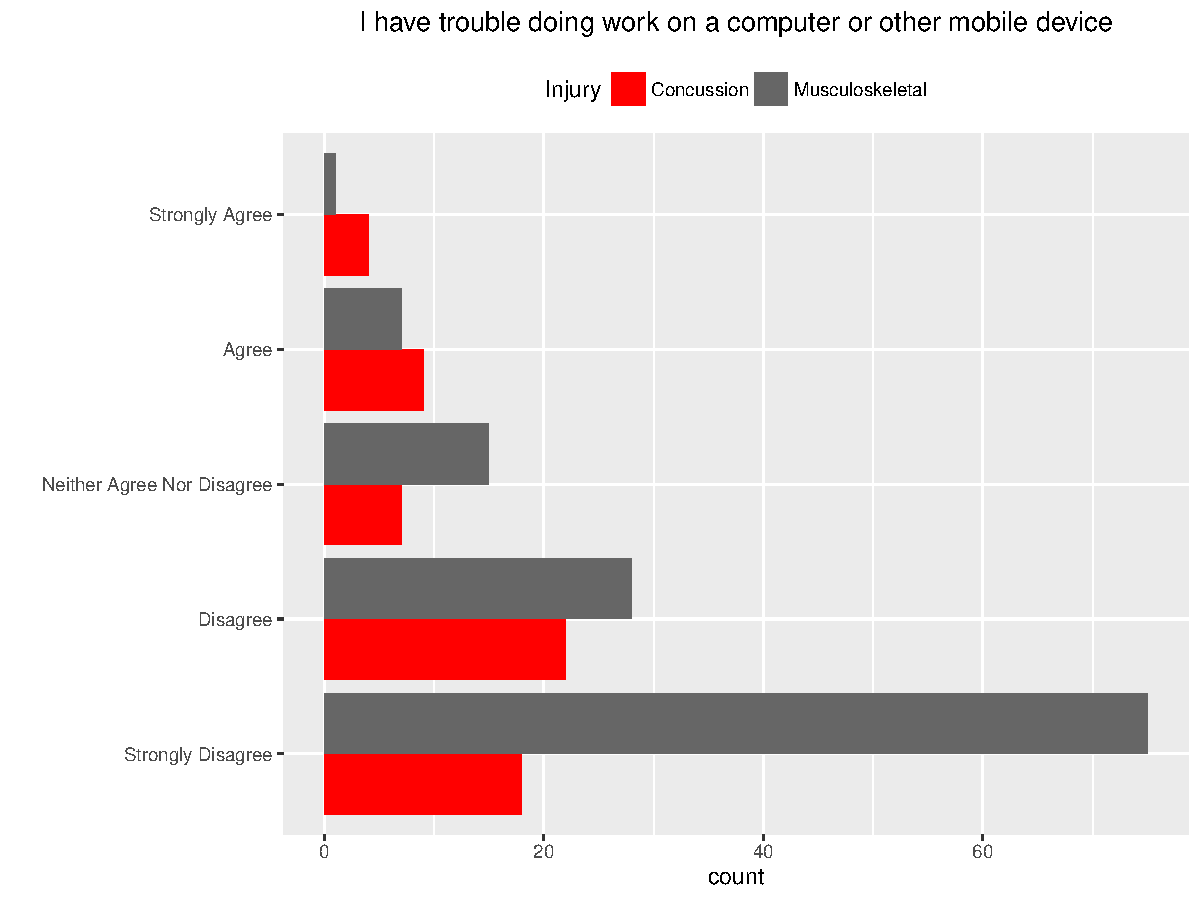
\includegraphics[width=0.5\linewidth]{Q5_3_18_barPlot.pdf} \\
% \end{figure}
% 
% \begin{figure}[H]
% 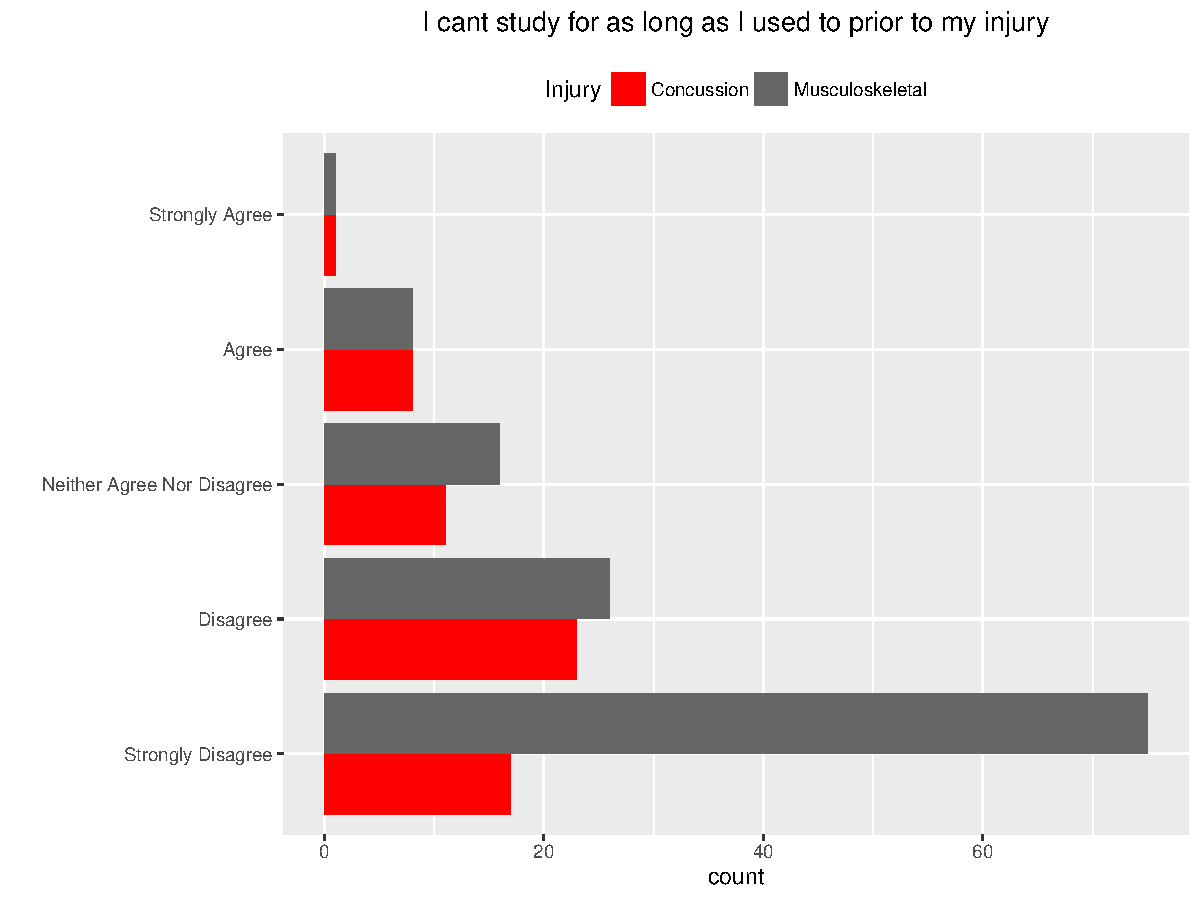
\includegraphics[width=0.5\linewidth]{Q5_3_19_barPlot.pdf}
% 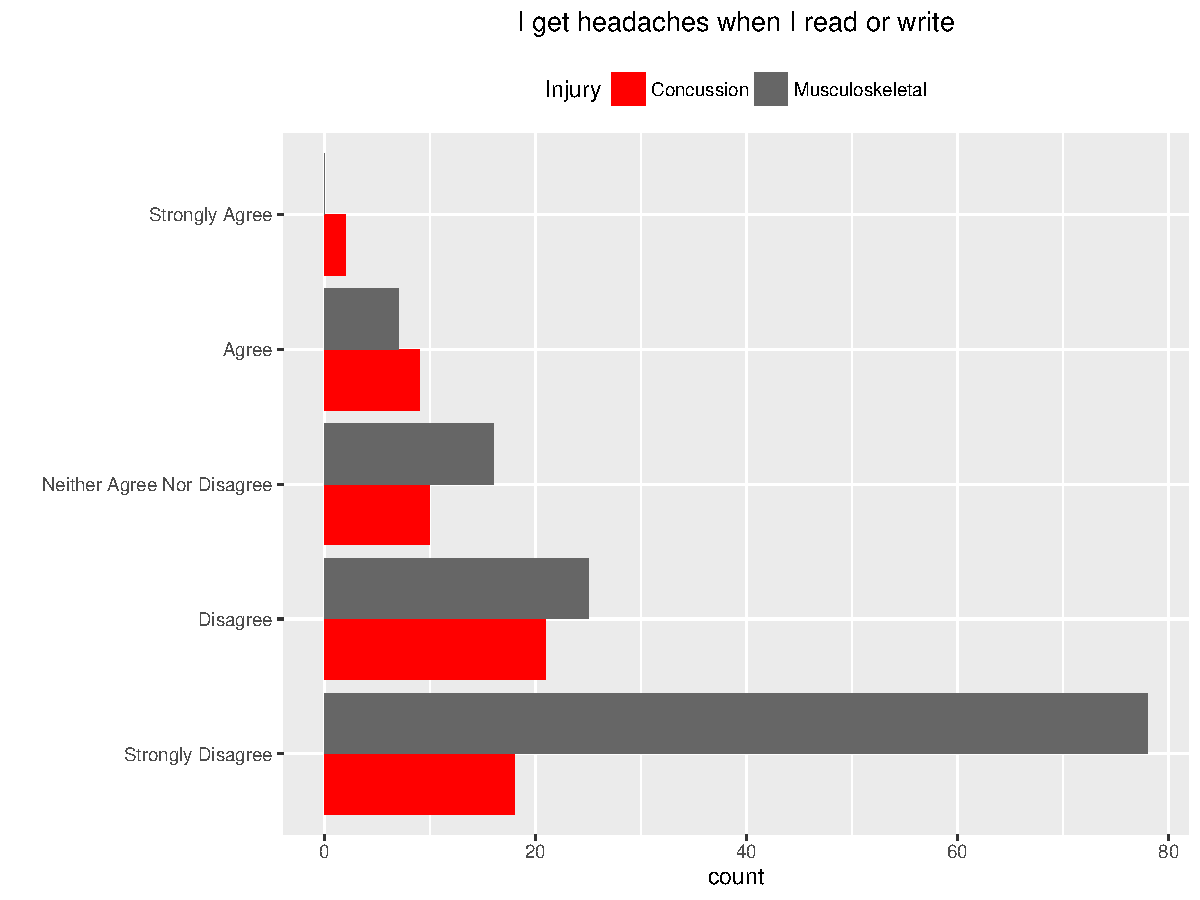
\includegraphics[width=0.5\linewidth]{Q5_3_20_barPlot.pdf} \\
% 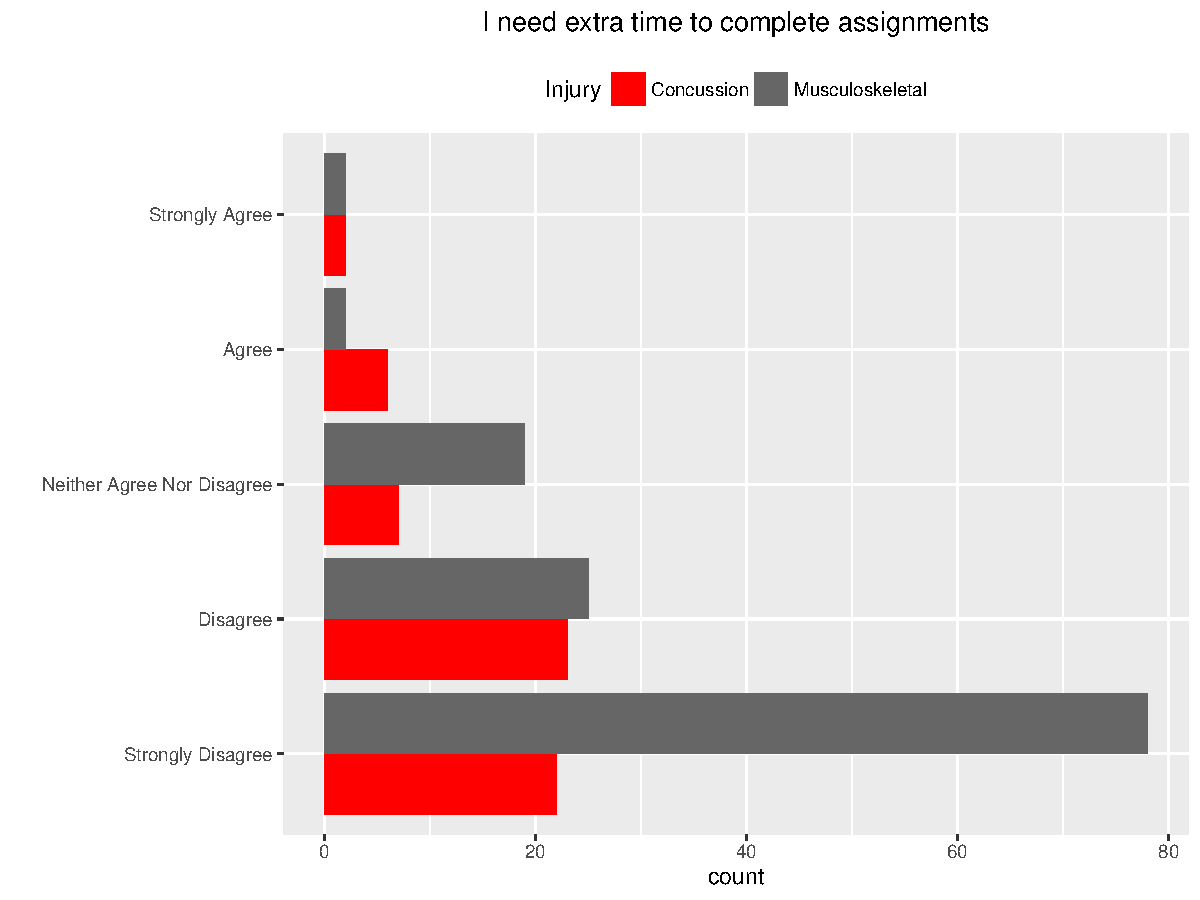
\includegraphics[width=0.5\linewidth]{Q5_3_21_barPlot.pdf}
% 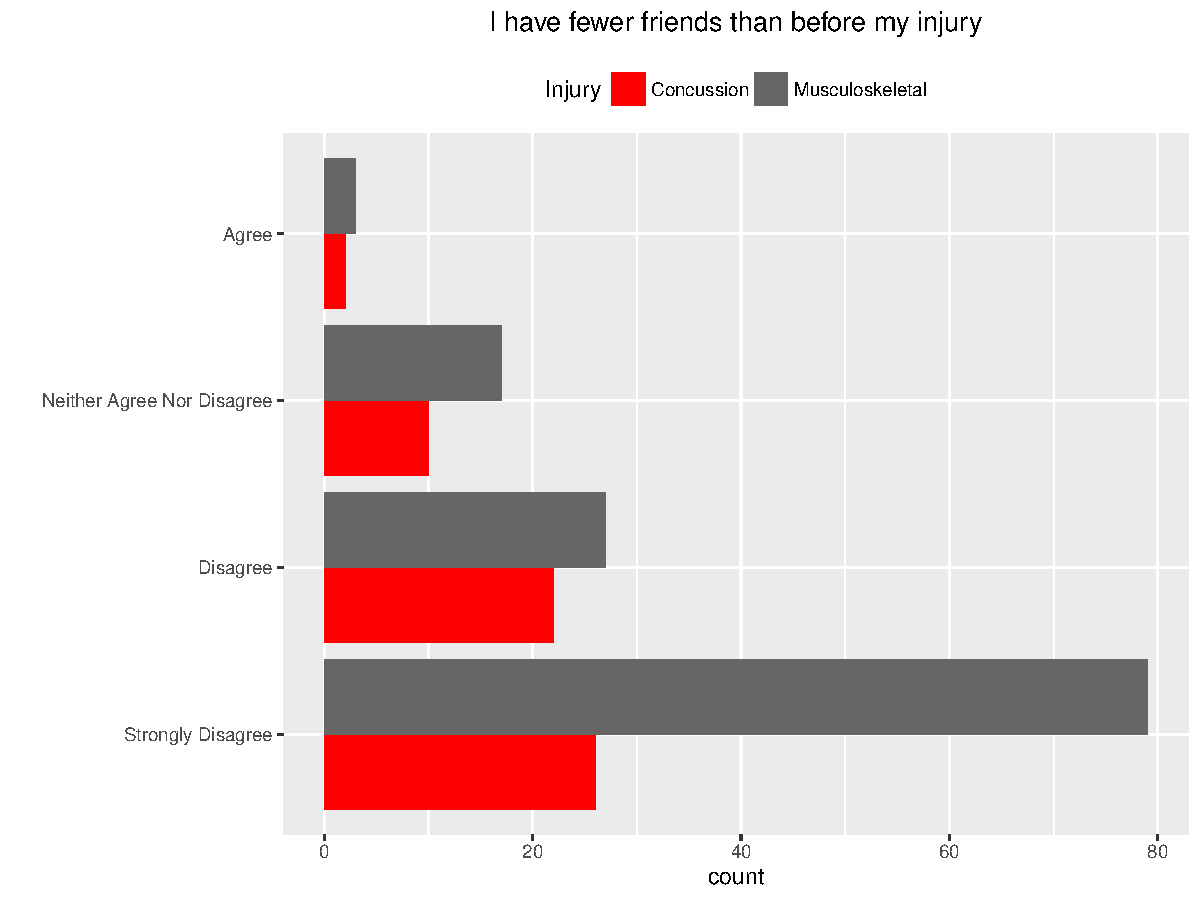
\includegraphics[width=0.5\linewidth]{Q5_3_22_barPlot.pdf}
% \end{figure}

All computations were done using the statistical software R, version 3.3.1.

\subsubsection*{Limitations}
The summary and statistical findings, although interesting, have some limitations. The sample size was 76, and out of them 8 students did not respond to the question on self-reporting, further reducing the sample size to 68 students. Further analysis is necessary to assert if these non-respondents could be asserted as "missing-at-random". More respondents with information like the reason for injury, their activities, etc, would improve the predictive power of this model. A more balanced sample, in terms of the predictors would improve the robustness of the results. For example, if more males responded to the survey it would improved the gender balance. 



\end{document}
